% !TEX root = ./document.tex

\documentclass[a4paper, spanish]{article}

\usepackage{mystyle}
\usepackage{myvars}

\begin{document}

  \maketitle

  \begin{itemize}
    \item \textbf{Archivo}: \texttt{weight-loss.csv}
    \item \textbf{Serie}: [TODO].
  \end{itemize}

  \section{Etapa de identificación}

    \paragraph{}
    [TODO]

    \begin{figure}
      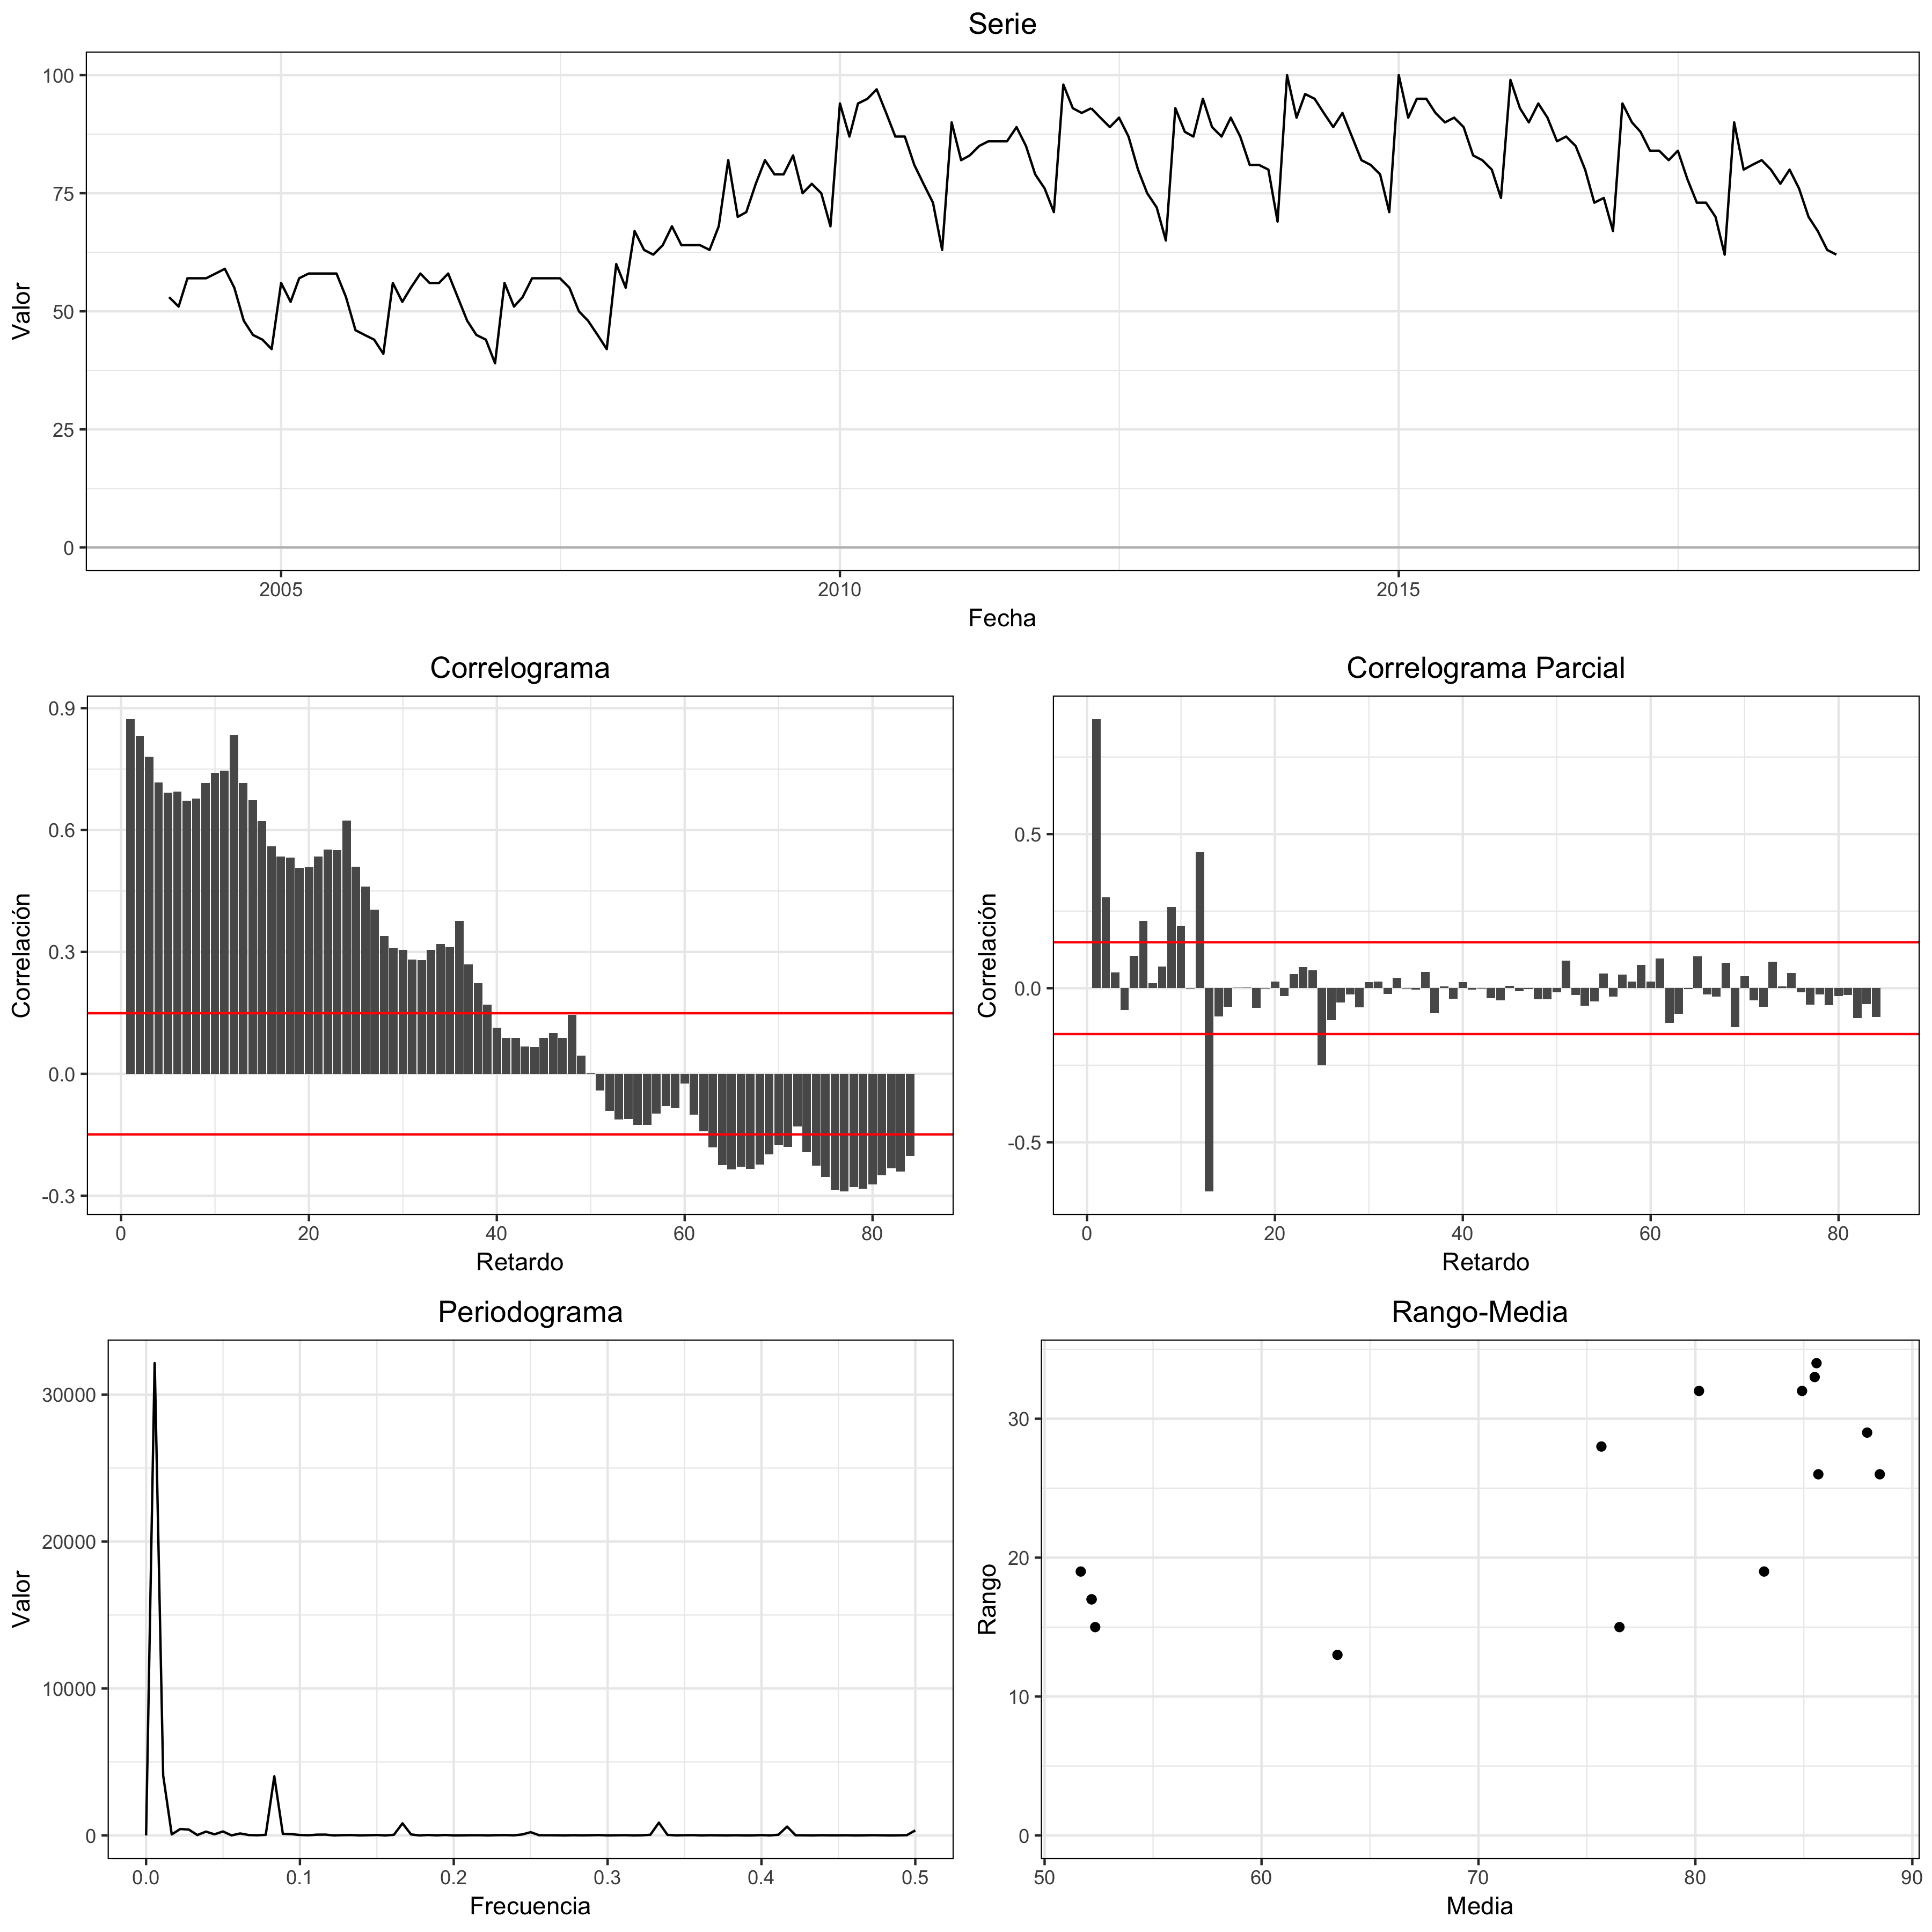
\includegraphics[width=\textwidth,height=\textheight,keepaspectratio]{weightloss}
      \caption{[TODO]}
      \label{}
    \end{figure}

    \paragraph{}
    [TODO]

    \begin{figure}
      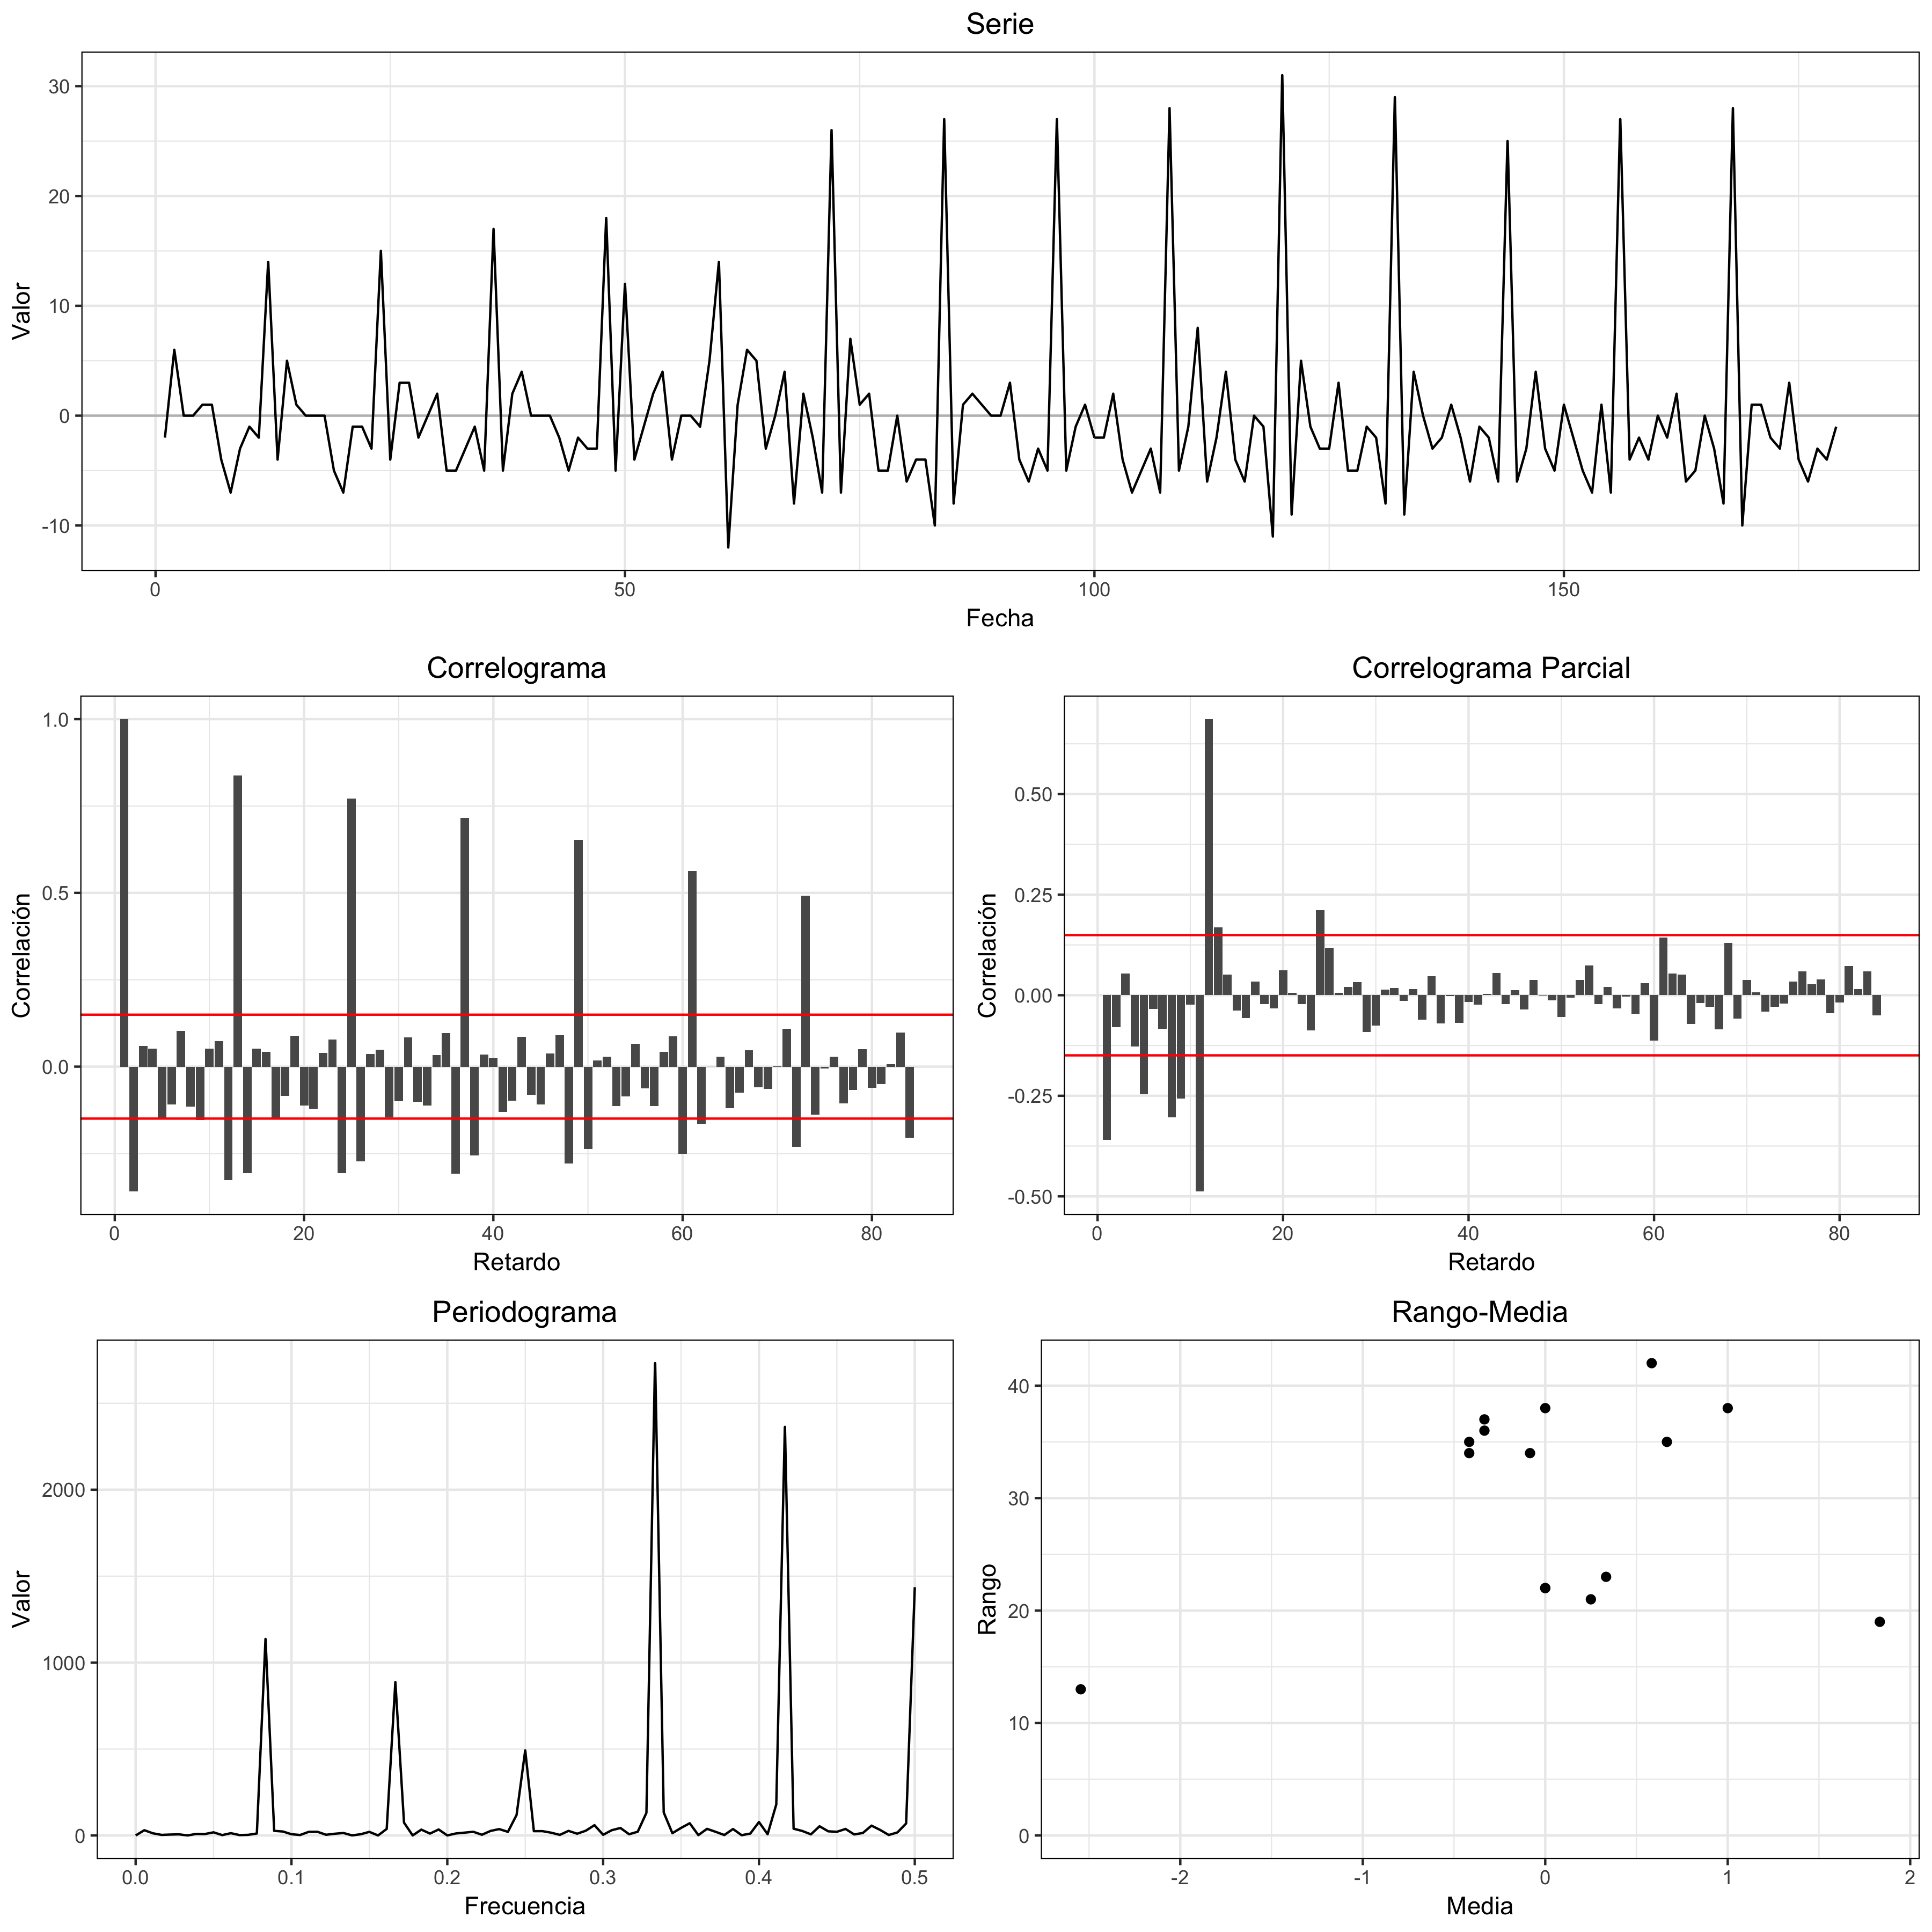
\includegraphics[width=\textwidth,height=\textheight,keepaspectratio]{weightloss-diff-1}
      \caption{[TODO]}
      \label{}
    \end{figure}

    \paragraph{}
    [TODO]

    \begin{figure}
      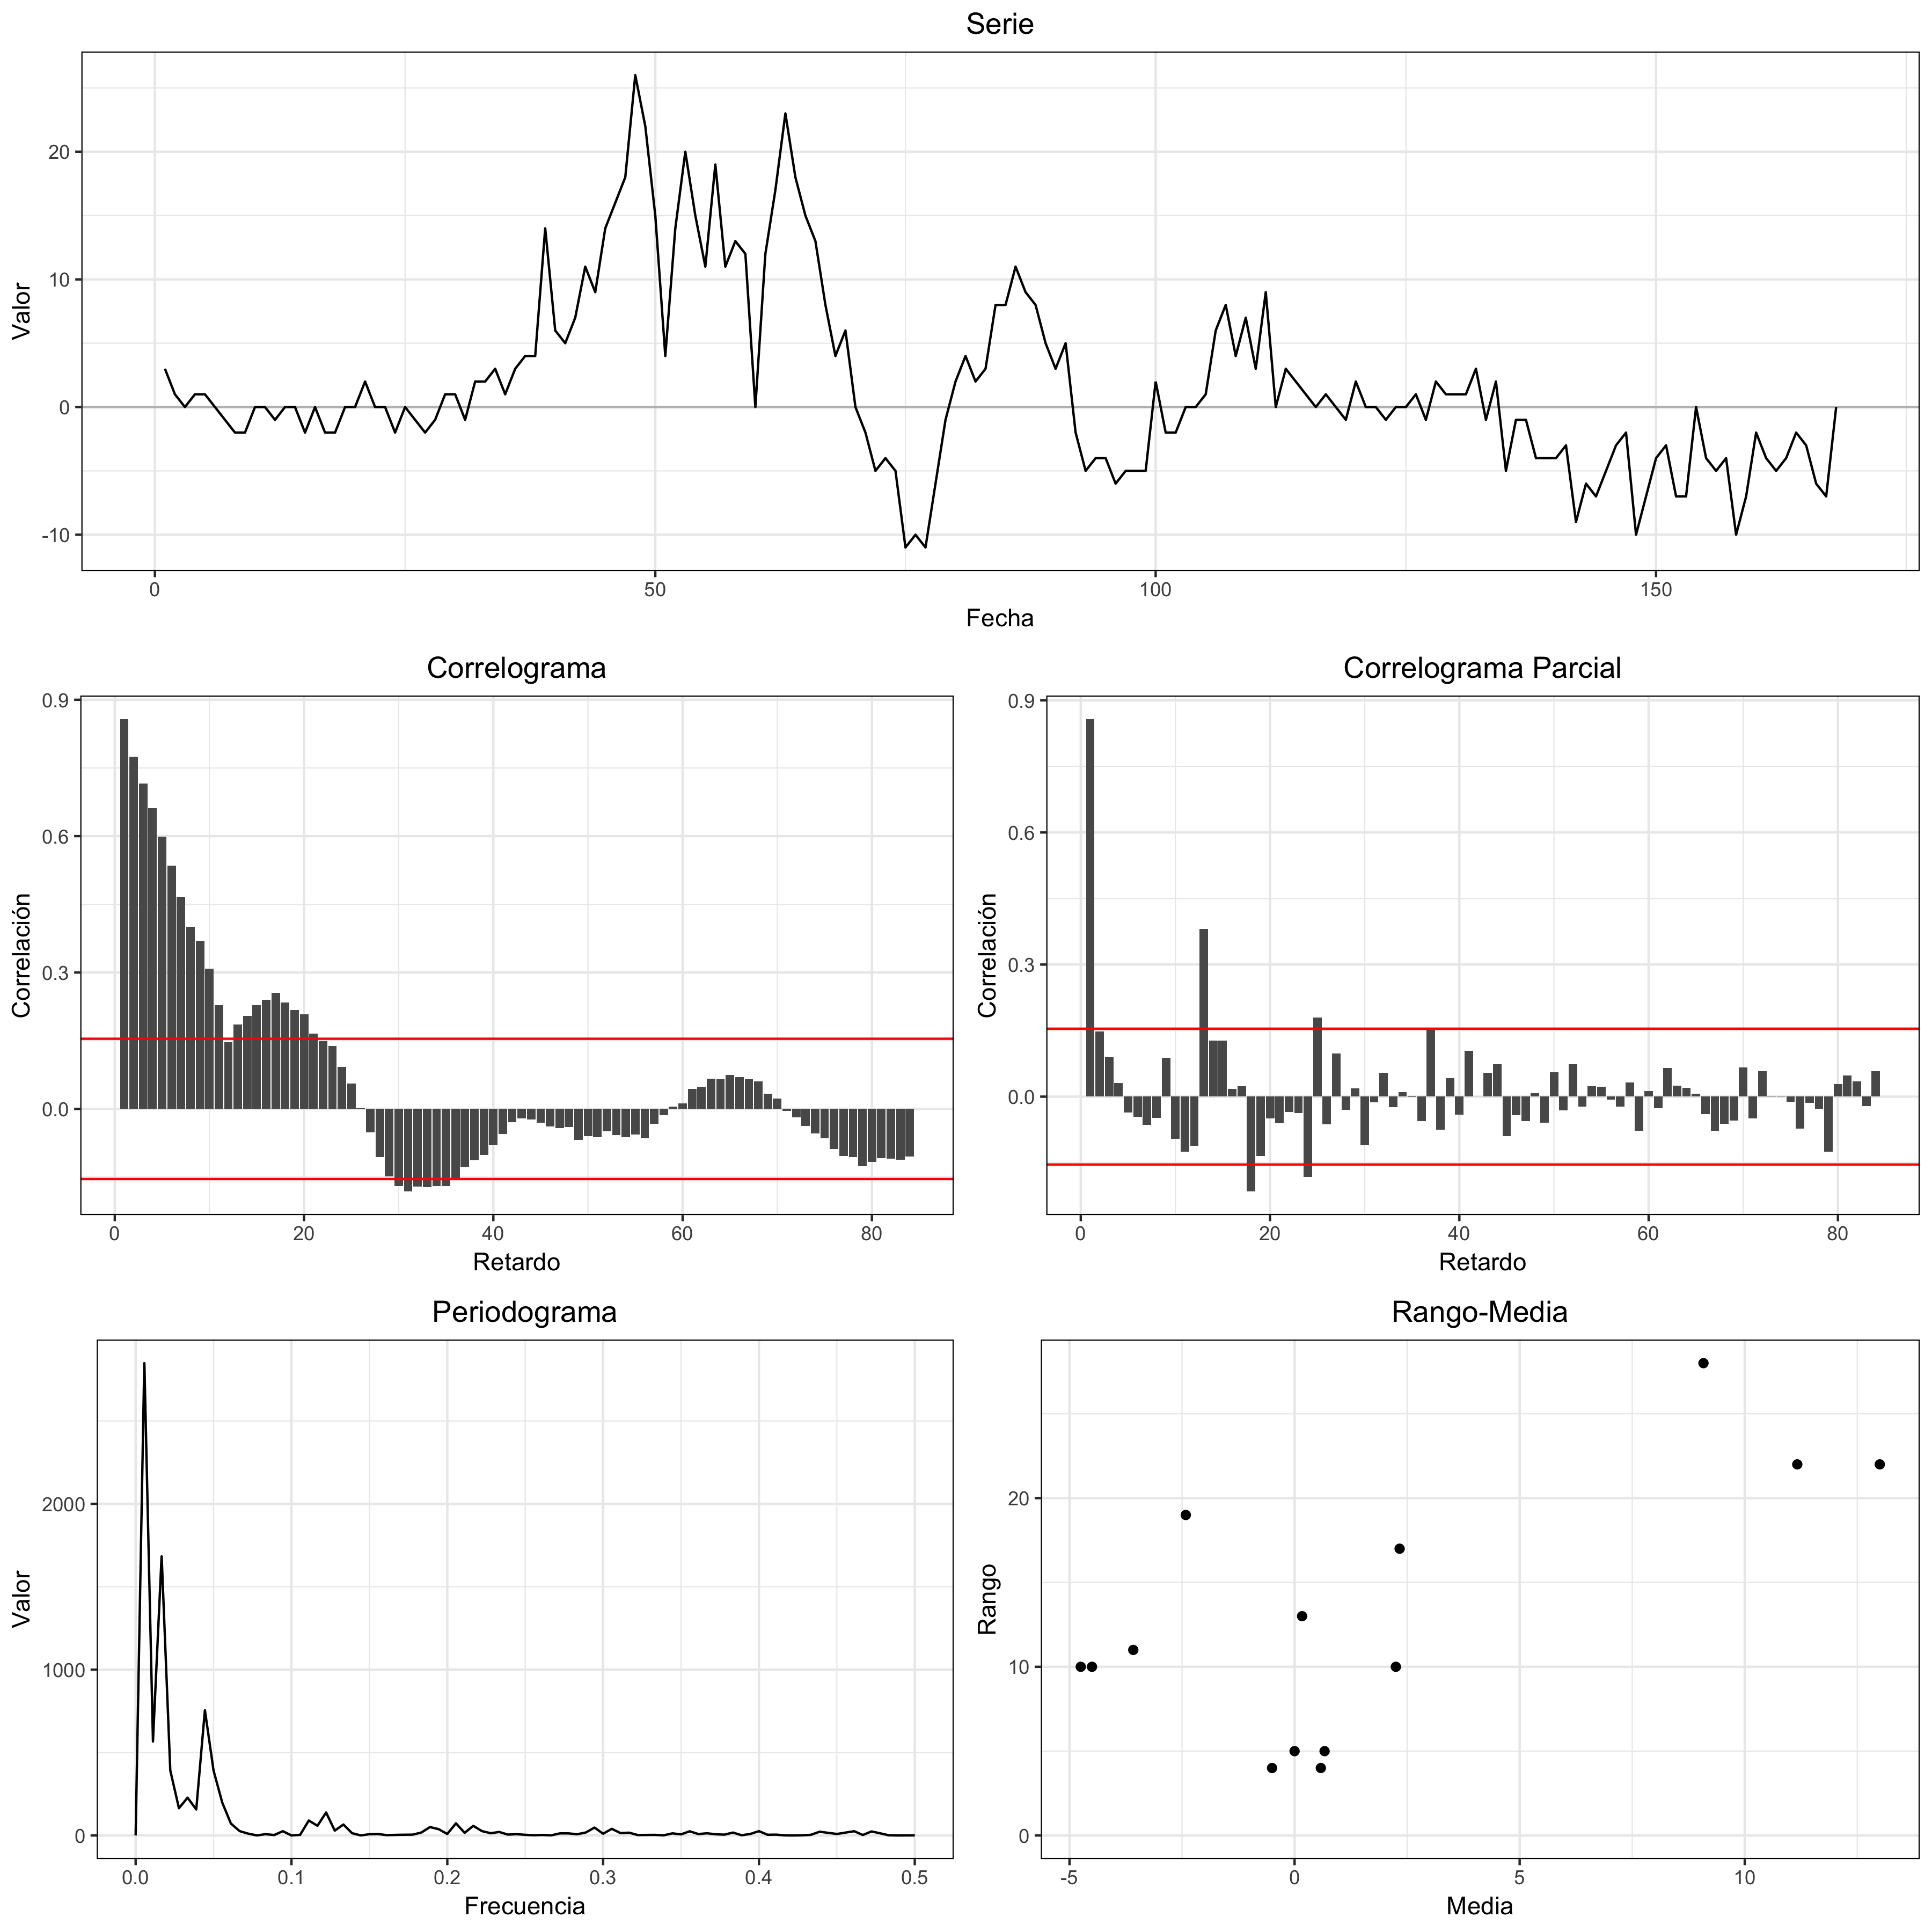
\includegraphics[width=\textwidth,height=\textheight,keepaspectratio]{weightloss-diff-12}
      \caption{[TODO]}
      \label{}
    \end{figure}

    \paragraph{}
    [TODO]

    \begin{figure}
      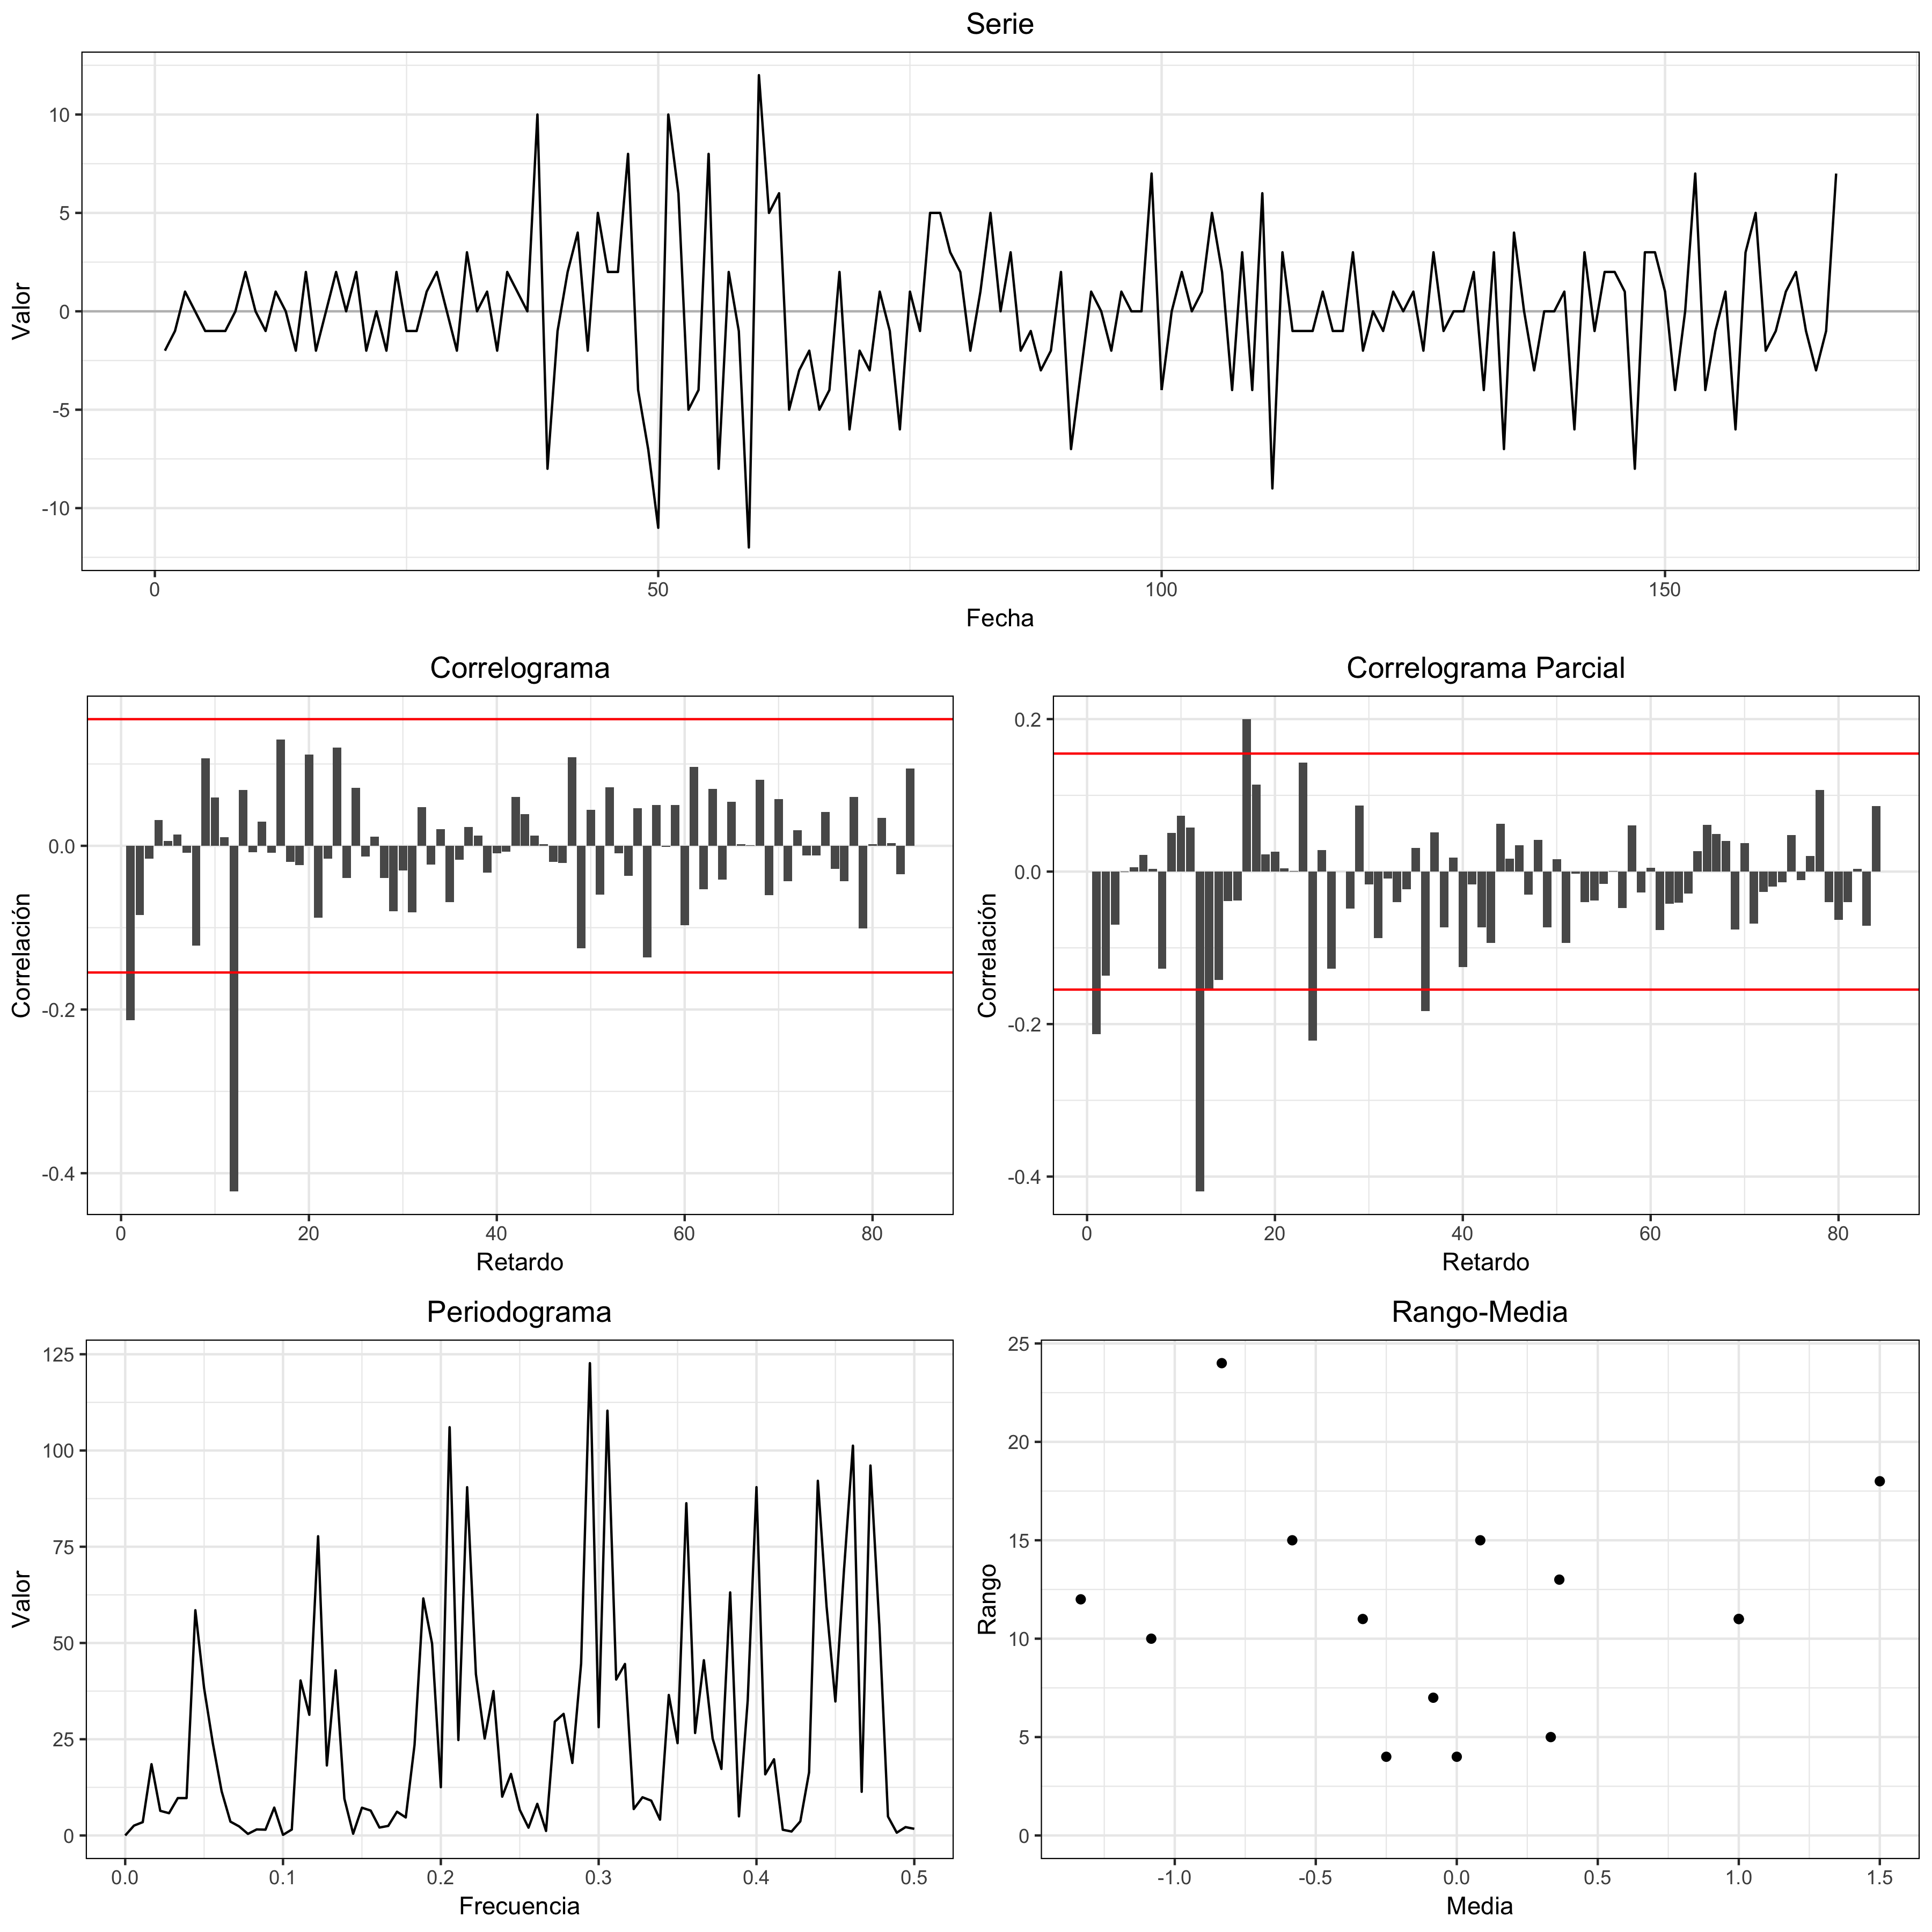
\includegraphics[width=\textwidth,height=\textheight,keepaspectratio]{weightloss-diff-1-12}
      \caption{[TODO]}
      \label{}
    \end{figure}

    \paragraph{}
    [TODO]

  \section{Etapa de estimación y validación}

    \paragraph{}
    [TODO]

  \section{Comparación de modelos}

    \paragraph{}
    [TODO]

  \section{Predicción}

    \paragraph{}
    [TODO]

  \appendix
  \section{Código Fuente}

    \paragraph{}
    [TODO]


    \begin{listing}[H]
        \centering
        \inputminted{R}{./res/code/weight-loss.r}
        \caption{[TODO]}
        \label{}
      \end{listing}
\end{document}
